\documentclass[problem]{mcs}

\begin{pcomments}
  \pcomment{PS_TA_recitation_graph_coloring}
  \pcomment{from: S09.ps6}
\end{pcomments}

\pkeywords{
  graph_coloring
}

%%%%%%%%%%%%%%%%%%%%%%%%%%%%%%%%%%%%%%%%%%%%%%%%%%%%%%%%%%%%%%%%%%%%%
% Problem starts here
%%%%%%%%%%%%%%%%%%%%%%%%%%%%%%%%%%%%%%%%%%%%%%%%%%%%%%%%%%%%%%%%%%%%%
\newcommand{\TAonename}{Eli}
\newcommand{\TAtwoname}{Megumi}
\newcommand{\TAthreename}{Rich}
\newcommand{\TAfourname}{Tom}
\newcommand{\TAfivename}{Stav}
\newcommand{\TAsixname}{Liz}
\newcommand{\TAsevenname}{Oscar}
\newcommand{\TAeightname}{Stephanie}
\newcommand{\TAninename}{David}


\begin{problem} 
Math for Computer Science is often taught using recitations.  Suppose
it happened that 8 recitations were needed, with two or three staff
members running each recitation.  The assignment of staff to
recitation sections is as follows:

\begin{itemize}
\item R1:  \TAonename, \TAtwoname, \TAthreename \\
\item R2:  \TAonename, \TAeightname, \TAninename\\
\item R3:  \TAtwoname, \TAfivename\\
\item R4:  \TAsixname, \TAeightname, \TAsevenname\\
\item R5:  \TAsixname, \TAfourname, \TAninename\\
\item R6:  \TAfourname, \TAfivename\\
\item R7:  \TAfourname, \TAeightname\\
\item R8:  \TAtwoname, \TAfivename, \TAninename
\end{itemize}

Two recitations can not be held in the same 90-minute time slot if some
staff member is assigned to both recitations.  The problem is to determine
the minimum number of time slots required to complete all the recitations.

\begin{problemparts}

\problempart Recast this problem as a question about coloring the
vertices of a particular graph.  Draw the graph and explain what the
vertices, edges, and colors represent.

\begin{solution}
Each vertex in the graph below represents a recitation
section.  An edge connects two vertices if the corresponding
recitation sections share a staff member and thus can not be scheduled
at the same time.  The color of a vertex indicates the time slot of
the corresponding recitation.

\begin{center}
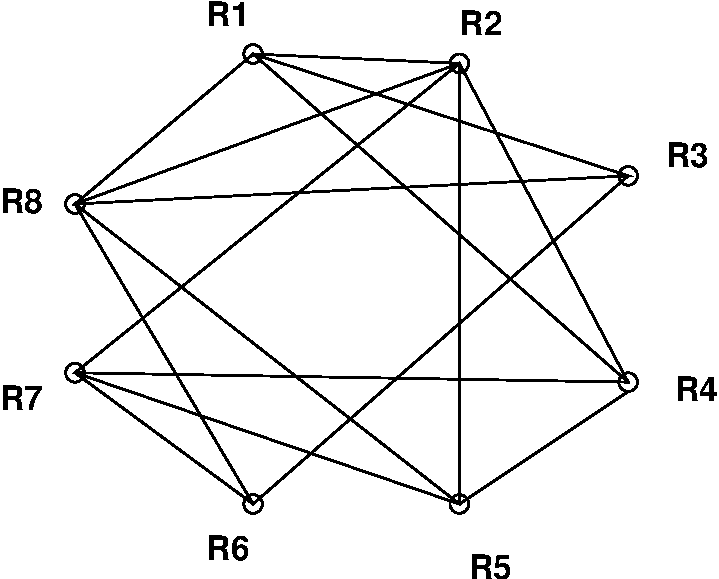
\includegraphics[height=2in]{figures/S09_PS6_schedule.pdf}
\end{center}
\end{solution}

\problempart
Show a coloring of this graph using the fewest possible
colors.  What schedule of recitations does this imply?

\begin{solution}
Four colors are necessary and sufficient. To see why they
are \emph{sufficient}, consider the coloring:
\begin{center}
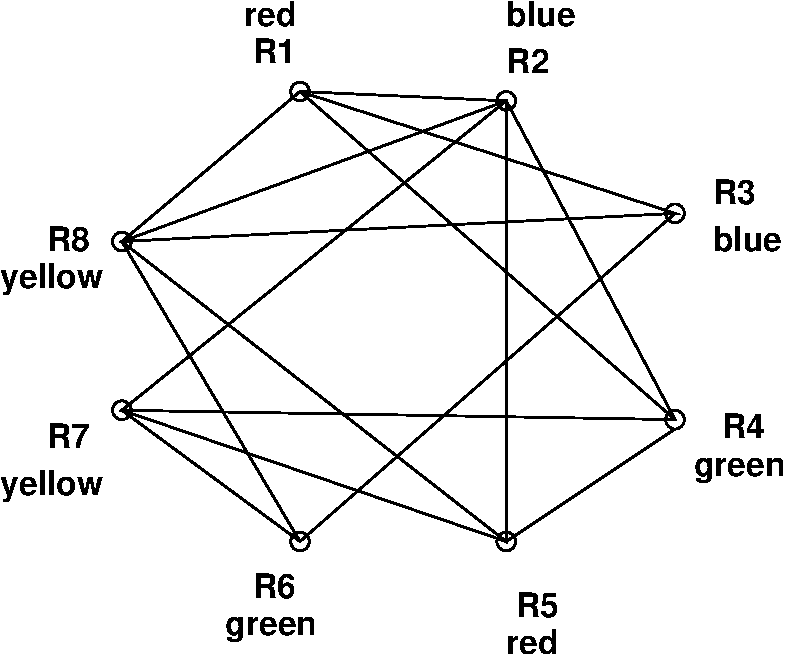
\includegraphics[height=2in]{figures/S09_PS6_schedule_colored.pdf}
\end{center}
This corresponds to the following assignment of recitations to four
time slots:
\begin{enumerate}

\item R1, R5

\item R2, R3

\item R4, R6

\item R7, R8

\end{enumerate}
Other schedules are also possible.

To see why 4 colors are \emph{necessary}, look at the subgraph defined
by the vertices for R2, R4, R5, and R7.  This is the complete graph on 4
vertices, and it obviously needs 4 colors.
\end{solution}

\end{problemparts}

\end{problem}

%%%%%%%%%%%%%%%%%%%%%%%%%%%%%%%%%%%%%%%%%%%%%%%%%%%%%%%%%%%%%%%%%%%%%
% Problem ends here
%%%%%%%%%%%%%%%%%%%%%%%%%%%%%%%%%%%%%%%%%%%%%%%%%%%%%%%%%%%%%%%%%%%%%

\endinput
